%==================================================================================================
\subsection{\textit{Large Eddy Simulation}} \label{LES}
%==================================================================================================

Em escoamentos com elevados números de Reynolds, observa-se a formação de vórtices em um amplo espectro de escalas, o que torna a simulação direta desses escoamentos computacionalmente inviável, uma vez que se exigem altas resoluções da malha do fluido para capturar todos os efeitos. Nesse sentido, a simulação de grandes vórtices (\textit{Large Eddy Simulation} - LES) surge como uma alternativa para se obter resultados próximos aos da simulação direta, porém com um custo computacional reduzido.

O LES originou-se do trabalho de \citeonline{smagorinsky1963general} no intuito de se estudar simulações de camadas limite atmosféricas e tendo o coeficiente de Smagorinsky estimado por \citeonline{deardorff1971magnitude} ao estudar escoamentos em canais. A ideia central do modelo parte da consideração de que o escoamento pode ser bem caracterizado por meio de uma separação de escalas, na qual as grandes escalas são responsáveis pela transferência da energia cinética, sendo influenciadas diretamente pela natureza do escoamento, assim como pelas condições de contorno, enquanto as pequenas escalas são responsáveis pela dissipação de energia e possuem propriedades isotrópicas e homogêneas no escoamento. Assim, o modelo de Smagorinsky consiste em uma decomposição do campo de velocidades em duas parcelas, uma de grandes escalas e outra de pequenas escalas, sendo a parcela de pequenas escalas modelada por um termo viscoso, o qual é determinado a partir de um modelo de viscosidade de vórtice.

Assim, a decomposição das variáveis do problema ($\phi$) se dá por $\phi=\bar{\phi}+\phi'$, em que $\bar{\phi}$ é a parcela de grandes escalas e $\phi'$ é a parcela de pequenas escalas. Tal separação é dada a partir da consideração de um filtro, definido como a convolução integral de uma função $\filter$, dita como filtro, com a variável $\phi$ \cite{germano1991dynamic,hughes2000large,moeng2015large,katopodes2019free}:

\begin{equation}
    \bar{\phi}=\int_{\Dfil}{\filter(\BB{y}-\yfil,t)\phi(\yfil,t)d\yfil}\text{,}
\end{equation}

\noindent em que $\Dfil$ é um subdomínio de $\Omega$ que determina a abrangência do filtro, $\yfil$ é um ponto na vizinhança de $\BB{y}$ e $\filter$ é o filtro. \citeonline{hughes2000large} apresentam ainda uma possibilidade de abrangência de filtro dada por:

\begin{equation}
    \Dfil=\left\{\yfil\in\mathbb{R}^{n_{sd}}|\rho_\Delta(\BB{y},\yfil)<\Delta/2\right\}\text{,}
\end{equation}

\noindent na qual $\Delta/2$ é o raio de abrangência do filtro centrado em $\BB{y}$ e $\rho_\Delta$ é a distância Euclidiana de $\yfil$ à $\BB{y}$.

Assim, um filtro $\filter$ deve ser capaz de remover as altas frequências na representação de Fourier e deve ser escolhido de forma a obedecer algumas propriedades, \ie\ a condição de homogeneidade: $\filter(\BB{y},\yfil,t)=\filter(\BB{y}-\yfil,t)$, a condição de isotropia: $\filter(\BB{y}-\yfil,t)=\filter(\rho_\Delta,t)$, a condição de normalização:

\begin{equation}
    \int_{\Dfil}{\filter(\BB{y}-\yfil,t)d\yfil}=1
\end{equation}

\noindent e deve possuir um suporte compacto, ou seja, sua influência deve diminuir com o aumento da distância de seu centro.

Dessa maneira, algumas propriedades são garantidas, como a conversão da operação de convolução em multiplicação em um espaço de Fourier, a qual é dada por:

\begin{subequations}
    \begin{equation}
        \Fourier{\bar{\phi}}(\BB{k},t)=\Fourier{\filter}(\BB{k},t)\Fourier{\phi}(\BB{k},t)\text{ e}
    \end{equation}
    \begin{equation}
        \Fourier{\phi'}(\BB{k},t)=(1-\Fourier{\filter}(\BB{k},t))\Fourier{\phi}(\BB{k},t)\text{,}
    \end{equation}
\end{subequations}

\noindent em que o sobrescrito $\mathcal{F}$ representa a transformação de Fourier. Além disso, a filtragem é uma operação linear, ou seja, $\bar{\phi}+\bar{\psi}=\overline{\phi+\psi}$ e $\alpha\bar{\phi}=\overline{\alpha\phi}$, em que $\alpha$ é uma constante. Já em domínios ilimitados, cujo filtro possui abrangência constante, tem-se a comutatividade da filtragem com a diferenciação, ou seja, $\bar{\Ny\phi}=\Ny\bar{\phi}$.

\citeonline{katopodes2019free} apresenta algumas possibilidades de filtro, os quais são apresentados na Tabela \ref{tab:filters}, assim como sua respectiva transformada de Fourier. A variável $k$ representa o número de onda. A Figura \ref{fig:Filters} apresenta graficamente o comportamento dos filtros apresentados na Tabela \ref{tab:filters}.

\begin{table}[h!]
    \centering
    \caption{Filtros utilizados em LES.}
    \begin{tabular}{lll}
        \hline
        Filtro              & Função                                                                                                                                             & Transformada de Fourier                                                                                                  \\\hline
        \textit{Box filter} & $\filter(\rho_\Delta)=\left\{\begin{array}{ll}\frac{1}{\Delta} & \text{ se }\rho_\Delta\leq\Delta/2 \\0& \text{ caso contrário}\end{array}\right.$ & $\Fourier{\filter}(k)=\frac{\sin{(k\Delta/2)}}{k\Delta/2}$                                                               \\
        Filtro gaussiano    & $\filter(\rho_\Delta)=\sqrt{\frac{\gamma_g}{\pi\Delta^2}}e^{-\frac{\gamma\rho_\Delta^2}{\Delta^2}}$                                                & $\Fourier{\filter}(k)=e^{-\frac{k^2\Delta^2}{4\gamma}}$                                                                  \\
        Filtro espectral    & $\filter(\rho_\Delta)=\frac{\sin{(k_c\rho_\Delta)}}{k_c\rho_\Delta}$                                                                               & $\Fourier{\filter}(k)=\left\{\begin{array}{ll} 1 & \text{ se }|k|\leq k_c \\0& \text{ caso contrário}\end{array}\right.$ \\\hline
    \end{tabular}
    \\Fonte: \citeonline{katopodes2019free} - Adaptado.
    \label{tab:filters}
\end{table}

\begin{figure}[h!]
    \centering
    \caption{Comportamento dos filtros apresentados na Tabela \ref{tab:filters}.}
    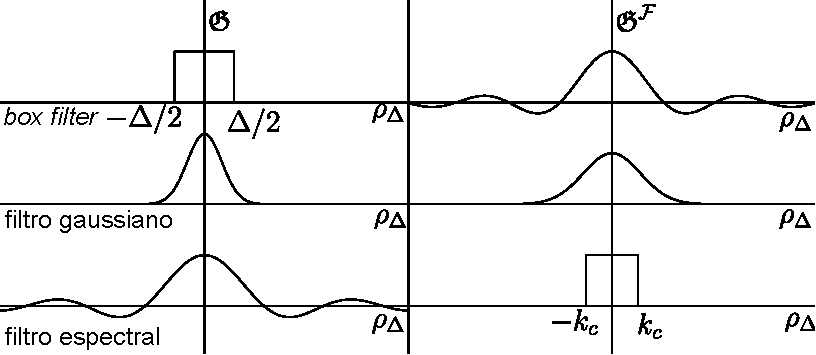
\includegraphics[width=.85\linewidth]{Figuras/filtros.pdf}
    \\Fonte: Autoria Própria (\the\year).
    \label{fig:Filters}
\end{figure}

O valor $\gamma_g$ observado no filtro gaussiano é uma constante, comumente atribuída com o valor de 6,0. Já o parâmetro $k_c$ é o número de onda de corte, dado por $k_c=\pi/\Delta$. Dentre os filtros apresentados, percebe-se que tanto o \textit{box filter} quanto o filtro gaussiano possuem suporte compacto no espaço físico, porém não possuem suporte compacto no espaço de Fourier, o que pode gerar problemas numéricos. Já o filtro espectral possui suporte compacto no espaço de Fourier, porém não possui suporte compacto no espaço físico.

Dessa maneira, é possível separar os efeitos das grandes escalas e das pequenas escalas, o que é ilustrado na Figura \ref{fig:EfeitoFiltragem} para uma distribuição de velocidade $\BB{u}$.

\begin{figure}[h!]
    \centering
    \caption{Efeito da filtragem sobre um campo de velocidades $\BB{u}$.}
    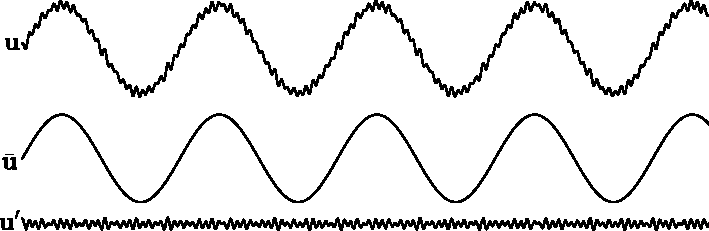
\includegraphics[width=.75\linewidth]{Figuras/efeito_filtragem.pdf}
    \\Fonte: \citeonline{hughes2000large} - Adaptado.
    \label{fig:EfeitoFiltragem}
\end{figure}

Assim, em uma descrição Euleriana, pode-se obter as equações de Navier-Stokes filtradas:

\begin{subequations}
    \begin{align}
         & \rho\bigpar{\dot{\BBB{u}}+\Ny\cdot(\overline{\BB{u}\otimes\BB{u}})-\BBB{f}}-\Ny\cdot\bar{\tens}=\BB{0} &  & \text{ em }\Omega\text{,} \\
         & \Ny\cdot\BBB{u}=0                                                                                      &  & \text{ em }\Omega\text{.}
    \end{align}
\end{subequations}

Pode-se perceber que o termo convectivo impede a completa separação dos termos $\BBB{u}$ e $\BB{u}'$ devido à sua natureza altamente não-linear. Por conta disso a parcela não filtrada não pode ser ignorada nesse problema, sendo necessário realizar algumas manipulações algébricas. Sabendo-se que $\BB{u}=\BBB{u}+\BB{u}'$, pode-se reescrever a equação da conservação da quantidade de movimento como:

\begin{equation}
    \rho\bigpar{\dot{\BBB{u}}+\Ny\cdot(\overline{(\BBB{u}+\BB{u}')\otimes(\BBB{u}+\BB{u}')})-\BBB{f}}-\Ny\cdot\bar{\tens}=\BB{0}
\end{equation}

Nesse sentido, surgirão termos cruzados entre $\BBB{u}$ e $\BB{u}'$, os quais serão condensados em um tensor de subescala (\textit{Subgrid-Scale} - SGS) $\BB{T}$ dado por \cite{piomelli1999large,hughes2000large}:

\begin{equation}
    \BB{T}=\BBB{u}\otimes\BBB{u}-\overline{\BB{u}\otimes\BB{u}}=-\bigpar{\BB{L}+\BB{C}+\BB{R}}\text{,}
\end{equation}

\noindent no qual $\BB{L}=\overline{\BBB{u}\otimes\BBB{u}}-\BBB{u}\otimes\BBB{u}$ é o tensor de Leonard, que representa as interações entre as grandes escalas, podendo ser determinado explicitamente e utilizado para análise de erros, $\BB{C}=\overline{\BBB{u}\otimes\BB{u}'}+\overline{\BB{u}'\otimes\BBB{u}}$ é o tensor de termos cruzados, representando a interação entre as grandes e pequenas escalas e $\BB{R}=\overline{\BB{u}'\otimes\BB{u}'}$ é o tensor de tensões SGS de Reynolds, que representa a interação entre as pequenas escalas \cite{piomelli1999large}. Assim pode-se escrever:

\begin{equation}
    \rho\bigpar{\dot{\BBB{u}}+\Ny\cdot(\BBB{u}\otimes\BBB{u})-\Ny\cdot\BB{T}-\BBB{f}}-\Ny\cdot\bar{\tens}=\BB{0}\text{.}
\end{equation}

Aplicando a incompressibilidade e substituindo-se $\bar{\tens}$ pelo modelo constitutivo \eqref{eq:ModConst}, tem-se que:

\begin{equation}
    \rho\bigpar{\dot{\BBB{u}}+(\BBB{u}\cdot\Ny)\BBB{u}-\Ny\cdot\BB{T}-\BBB{f}}-\mu\Ny\cdot(\Ny\BBB{u}+\NyT\BBB{u})+\Ny p=\BB{0}\text{,}\label{eq:ConMasLES}
\end{equation}

\noindent ou, dividindo-se por $\rho$ e fazendo algumas manipulações tem-se que:

\begin{equation}
    \dot{\BBB{u}}+(\BBB{u}\cdot\Ny)\BBB{u}+\frac{\Ny p}{\rho}=\nu\Lapl\BBB{u}+\Ny\BB{T}+\BBB{f}\text{,}
\end{equation}

\noindent sendo $\Lapl(\cdot)=\Ny\cdot\Ny(\cdot)$ o operador laplaciano e $\nu=\mu/\rho$ a viscosidade cinemática.

Assim, o problema fica governado por:

\begin{equation}
    \left\{
    \begin{array}{ll}
        \dot{\BBB{u}}+(\BBB{u}\cdot\Ny)\BBB{u}+\frac{\Ny p}{\rho}=\nu\Lapl\BBB{u}+\Ny\cdot\BB{T}+\BBB{f} & \text{ em }\Omega\text{,} \\
        \Ny\cdot\BBB{u}=0                                                                                & \text{ em }\Omega\text{,}
    \end{array}
    \right.
\end{equation}

\noindent havendo ainda a necessidade de se determinar um tensor $\BB{T}$, em especial o seu tensor desviador:

\begin{equation}
    \dev{\BB{T}}=\BB{T}-\frac{1}{3}\tr{(\BB{T})}\BB{I}\text{,}
\end{equation}

\noindent que descreva adequadamente as interações entre diferentes escalas. Isso pode se tornar problemático uma vez que não se possui solução para as pequenas escalas. Uma forma de se fazer isso é através do modelo de viscosidade de vórtice de Smagorinsky \cite{smagorinsky1963general}, resultando no tensor:

\begin{equation}
    \bigpar{\BB{T}_S}=2\nu_T\deffil\text{,}
\end{equation}

\noindent sendo $\nu_T$ a viscosidade de vórtice SGS, dada por \cite{germano1991dynamic,piomelli1999large,hughes2000large,bailly2015turbulence,katopodes2019free}:

\begin{equation}
    \nu_T=(C_S\Delta)^2\norm{\deffil}\text{,}
\end{equation}

\noindent onde $C_S$ é a constante de Smagorinsky e $\norm{\deffil}$ é a magnitude do tensor taxa de deformação em escala grosseira, dada por:

\begin{equation}
    \norm{\deffil}=(2\deffil:\deffil)^{1/2}\text{.}
\end{equation}

Note que o tensor $\BB{T}_S$ é um tensor desviador, ou seja, $\BB{T}_S=\dev{\BB{T}_S}$.

%\citeonline{germano1991dynamic,hughes2000large} ainda fazem algumas constatações sobre o modelo de Smagorinsky, os quais destacam-se o fato de $\BB{T}_S$ não possuir um comportamento assintótico próximo às paredes, o que se esperaria de $\BB{T}$, os valores de $C_S$ na presença de cisalhamento médio causaram amortecimentos excessivos e o tensor $\BB{T}_S$ impede a energia de fluir entre diferentes escalas, podendo ser significante em alguns casos.
%
%Como tentativa de se resolver esses problemas, \citeonline{germano1991dynamic} propuseram assumir $C_S$ como uma função $C_S=C_S(\BB{y},t)$, permitindo, assim, que esse parâmetro se adapte para melhor modelar as pequenas escalas.

Para a determinação da constante de Smagorinsky, realiza-se inicialmente uma aproximação da amplitude espectral da energia cinética $E(k)$, dada sobre a superfície de uma esfera parametrizada de raio $k$, de acordo com \cite{hughes2000large}:

\begin{equation}
    E(k)\approx\alpha\varepsilon^{2/3}k^{-5/3}\text{,}\label{eq:Ek1}
\end{equation}

\noindent em que $\alpha$ é a constante de Kolmogoroff e $\varepsilon$ é a dissipação turbulenta. A Figura \ref{fig:EnergiaEspectral} apresenta graficamente o comportamento da energia espectral em função do raio $k$.

\begin{figure}[h!]
    \centering
    \caption{Energia espectral de Kolgomorov.}
    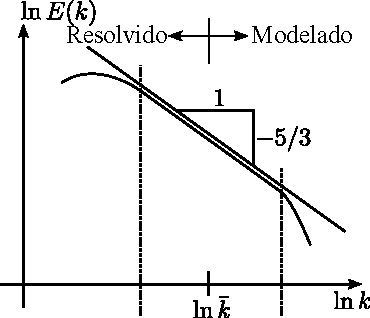
\includegraphics[width=0.4\linewidth]{Figuras/EnergiaEspectral.pdf}
    \\Fonte: \cite{hughes2000large} - Adaptado.
    \label{fig:EnergiaEspectral}
\end{figure}

O valor de $\norm{\deffil}$ é adotado como:

\begin{equation}
    \frac{1}{2}\norm{\deffil}=\int_0^{k_c}{k^2E(k)dk}\text{,}\label{eq:ndeffil1}
\end{equation}

\noindent sendo $k_c$ o limite de resolução.

Substituindo \eqref{eq:Ek1} em \eqref{eq:ndeffil1}, resolvendo a integral e fazendo algumas manipulações algébricas, tem-se que:

\begin{equation}
    \norm{\deffil}^3=\bigpar{\frac{3\alpha}{2}}^{3/2}k_c^2\varepsilon\text{.}
\end{equation}

Com isso, considerando também que a dissipação de energia cinética é igual àquela produzida, realiza-se o balanço da energia, obtendo-se:

\begin{equation}
    \varepsilon=\BB{T}_S:\deffil\text{.}
\end{equation}

\noindent Assim, fica possível obter expressões que relacionam os valores de $C_S$ $\Delta$ e $\nu_T$ com $k_c$:

\begin{equation}
    C_S\Delta=\bigpar{\frac{2}{3\alpha}}^{3/4}k_c^{-1}\text{ e}
\end{equation}

\begin{equation}
    \nu_T=\bigpar{\frac{2}{3\alpha}}\varepsilon^{1/3}k_c^{-4/3}\text{.}
\end{equation}

Segundo \citeonline{bailly2015turbulence} o valor de $k_c$ pode ser estimado como $k_c=\pi/\Delta$, o que leva à seguinte expressão para a constante de Smagorinsky:

\begin{equation}
    C_S=\frac{1}{\pi}\bigpar{\frac{2}{3\alpha}}^{3/4}\text{.}
\end{equation}

Com isso, um possível valor para a constante Kolmogoroff é $\alpha=1,4$, o que resulta em $C_S\approx0,18$. No entanto, segundo  \citeonline{hughes2000large,bailly2015turbulence,katopodes2019free}, valores de $C_S$ próximos à 0,10 conduzem a solução à resultados mais realistas.

\begin{comment}
%==================================================================================================
\subsubsection{Procedimento computacional} \label{LES-PC}
%==================================================================================================

Para a obtenção dos resultados, parte-se para a formulação variacional, em que se utiliza funções testes $\BB{w}$ e $q$, associadas às equações de conservação da quantidade de movimento e da continuidade, respectivamente. Assim, a forma fraca do problema LES é dada por:

\begin{equation}
    \begin{split}
        &\intDom{w_i\rho\bigpar{\dot{\ub}_i+\uub{j}\ub_{i,j}-\bar{f}_i}}+\intDom{\rho w_{i,j}T_{ij}}+\intDom{w_{i,j}\sigma_{ji}(\BB{\ub},\pb)}+\\
        &\intDom{q\ub_{i,i}}-\intNeumann{\rho w_iT_{ij}n_j}-\intNeumann{w_i\bar{h}_i}=0\text{.}
    \end{split}
\end{equation}

Substituindo o modelo constitutivo e o modelo de viscosidade de Smagorinsky tem-se que:

\begin{equation}
    \begin{split}
        &\intDom{w_i\rho\bigpar{\dot{\ub}_i+\uub{j}\ub_{i,j}-\bar{f}_i}}+\intDom{w_{i,j}(\mu+\rho\nu_T)(\uSim{\ub}{i}{j})}-\\
        &\intDom{w_{i,i}\pb}+\intDom{q\ub_{i,i}}-\intNeumann{w_i\bar{h}_i}=0\text{.}
    \end{split}
\end{equation}

\textcolor{purple}{
    No intuito de se obter uma solução estável, será considerado o elemento de Taylor-Hood P2P1 (aproximação quadrática para o campo de velocidades e linear para o campo de pressões) na formulação. Assim denomina-se $M$ as funções de forma para aproximação quadrática e $N$ para funções de forma lineares. Com isso, faz-se a aproximação das funções testes por meio das funções de forma, tendo como resultado os seguintes vetores de resíduo associados às equações de conservação de momento e da continuidade:
}
\textcolor{red}{1. Você deve deixar a formulação geral, e nos exemplos dizer o que você utilizou para obter resposta estável. Sugiro que desde o início (VMS) você diferencie as funções de forma de pressão e de velocidade (eu prefiro colocar um sobrescrito u e p ao invés de usar N e M). Aqui você deveria apresentar a formulação estabilizada, e nos exemplos você diz o que adotou para rodar. De qualquer forma, aqui ficou faltando colocar a estabilização para a convecção (SUPG) que sempre será necessária. Reveja o restante deste item com base nisso...}

\begin{subequations}
    \begin{equation}
        \begin{split}
            \bigpar{N_M}_i^a=&\intDom{M_a\rho\bigpar{\dot{\ub}_i+\uub{j}\ub_{i,j}-\bar{f}_i}}+\\
            &\intDom{M_{a,j}(\mu+\rho\nu_T)(\uSim{\ub}{i}{j})}-\intDom{M_{a,i}\pb}-\intNeumann{N_a\bar{h}_i}\text{ e}
        \end{split}
    \end{equation}
    \begin{equation}
        \bigpar{N_C}^a=\intDom{N_a\ub_{i,i}}\text{.}
    \end{equation}
    \label{eq:VetoresResiduo-LES}
\end{subequations}

Dessa forma procura-se determinar valores de $\ub$ e $\pb$ que anulem $N_M$ e $N_C$. Para esse fim utiliza-se o método de Newton-Raphson, em que as variáveis a serem determinadas são as acelerações e pressões nodais, sendo o integrador utilizado o $\alpha$-generalizado, apresentado na seção \ref{IT-VMS}. Desse modo tem-se os seguintes sub-blocos que compõem a matriz tangente:

\begin{subequations}
    \begin{equation}
        \begin{split}
            \der{(N_M)_i^a}{\dot{U}_j^b}=&\alpha_m\intDom{\rho M_aM_b}\dij+\beta_f\intDom{\rho M_aM_b\ub_{i,j}}+\\
            &\beta_f\intDom{\rho M_aM_{b,k}\uub{k}}\dij+\beta_f\intDom{(\mu+\rho\nu_T)M_{a,k}M_{d,k}}\dij+\\
            &\beta_f\intDom{(\mu+\rho\nu_T)M_{a,j}M_{b,i}}\text{,}
        \end{split}
    \end{equation}
    \begin{equation}
        \der{(N_M)_i^a}{P^b}=-\intDom{M_{a,i}N_b}\text{,}
    \end{equation}
    \begin{equation}
        \der{(N_C)^a}{\dot{U}_j^b}=\beta_f\intDom{N_aM_{b,j}}\text{ e}
    \end{equation}
    \begin{equation}
        \der{(N_C)^a}{P^b}=0\text{.}
    \end{equation}
    \label{eq:MatrizTangente-LES}
\end{subequations}

\noindent em que $\beta_f=\alpha_f\gamma\Delta t$.

Observa-se que o sub-bloco $\partial{\NC}/\partial\BB{P}$ está presente na diagonal principal do problema, possuindo valor nulo. Isso pode ser interpretado como a consideração das pressões como multiplicadores de Lagrange nessa formulação.

%Para obtenção da solução aproximada, utiliza-se um procedimento similar ao apresentado no algoritmo \ref{alg:MEF-VMS}, onde o comando \ref{alg:estabilizador} é alterado para computar o valor da viscosidade de vórtice, assim como os valores das componentes da matriz tangente e dos vetores de resíduo são alterados para se adequarem ao presente modelo.
\end{comment}